\section{Konzept 3}
\begin{figure}[h!]
	\centering
	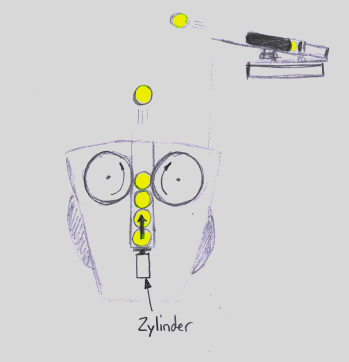
\includegraphics[width=0.4\textwidth]{../../fig/Wurfmaschine_Drehraeder.png}
	\caption{Aufbau mit zwei Rädern}
	\label{fig:drehradmaschine}
\end{figure}

\subsection{Idee}
Das dritte Konzept bedient sich einer unter Ballwurfmaschinen weit verbreiteten Methode Bälle zu beschleunigen. Zwei koaxial zueinander stehende Räder werden zum Drehen gebracht. Die Bälle müssen somit jeweils nur noch zwischen die Räder gebracht werden, um sich in Richtung der Drehrichtung zu beschleunigen.  

Als Variante dazu, würde sich ein Aufbau mit nur einem Drehrad anbieten.


\subsection{Annahmen}
Wir gehen davon aus,  dass die Grössenunterschiede der Bälle keinen signifikanten Einfluss auf die Wurfweite habe. Weiter schätzen wir die zwischen Rad und Ball entstehende Reibung als genügend stark für die Ballbeschleunigung ein.

\subsection{Vor- und Nachteile}
Vorteile:
-Schnelligkeit
-Einstellbare Wurfweite
-Einfacher Nachladeprozess

Nachteile:
-Bei einer Ausführung mit zwei Rädern müssen die Räder genau gleich schnell drehen, um am Ball entstehender Drall zu verhindern.
-Ungenügend genau einstellbare Drehzahlen könnten die Wurfweite schwer steuerbar machen. 
